%!TEX root = ./main.tex
So far, the main appeal of subjective expected utility (SEU) has been its conceptual simplicity, and the fact that it answers all decision problems in the same manner. 
In this chapter, we review some attempts at justifying SEU more formally, i.e. show that SEU logically follows from some simple, consensual principle.
When you hear someone say that ``Non-Bayesians are incoherent'', that ``a prior encapsulates the information available \emph{before} an experiment is made, so that the prior cannot depend on data", or that ``the posterior is the experimenter's updated belief after the experiment", or that ``Non-Bayesians violate the likelihood principle", they are all referring to one or the other of the formal justifications below. 
Not all these justifications are compatible, and none can really claim to be uniformly superior, so it is important to know upon what arguments you are resting your interpretation of the Bayesian procedure.

\section{Because you abide by the likelihood principle}
The ``formal" likelihood principle \citep{BeWo88} is a semi-formal justification that deals primarily with the estimation problem. 
We say \emph{half-formal} because some of the notions it deals with are left without rigorous mathematical definition, although this is not the main weak point \citep[Discussions]{BeWo88}. 

\subsection{The formal LP}
Consider two statistical experiments
$$
E_i=(\cY_i, \un{s}, \{p_i(\cdot\vert\vartheta), \vartheta\in\Theta\}), \quad i=1,2.
$$
Assume that for some realizations $\by_1$ and $\by_2$,
$$
p_1(\by_1\vert\cdot) \propto p_2(\by_2\vert \cdot).
$$
Note that we are using bold characters to insist on $\by_1$ and $\by_2$ being vectors concatenating (possibly many, of arbitrary dimension) observations, the label $i=1,2$ is only there to indicate which experiment we consider.
In particular, $\by_1$ and $\by_2$ may differ in dimension.

Now, assuming that there exists a quantity $\text{Ev}(E,x)$ that encapsulates the ``evidence on $\theta$ arising from $E$ and $x$", the formal LP principle is the requirement that
$$
\text{Ev}(E_1,\by_1) = \text{Ev}(E_2,\by_2).
$$
As a corollary, $\text{Ev}(E,\by)$ can depend on $x$ solely through $p(\by\vert\cdot)$.

\subsection{SEU satisfies the LP}
Letting $\cS = \cY^n\times\theta$, SEU satisfies the LP as long as the joint distribution over states has either $p_1$ or $p_2$ as its conditional of $\by$ given $\theta$.
Indeed, let
$$
p_i(s_i) = p_i(\by_i,\theta) = p_i(\by_i\vert\theta)\un{p(\theta)} = \un{Z} p_i(\theta\vert \by_i), \quad i=1,2.
$$
Note how we use a common prior. 
Then for $a:\cS\rightarrow\cZ$,
  $$ 
  \int L(a,s_1) \frac{p_1(\by_1\vert\theta)p(\theta)}{\un{Z}} \d\theta \propto \int L(a,s_2) \frac{p_2(\by_2\vert\theta)p(\theta)}{\un{Z}} \d\theta, 
  $$
  so that the posterior expected losses are the same in both experiments, and Bayes actions coincide.
  However, note that full expected utilities are different in general, 
  \begin{align*}
    \int L(a,s_1) p_1(\by_1\vert\theta)p(\theta) \unn{\d \by_1}\d\theta
    &\neq \int L(a,s_2) p_2(\by_2\vert\theta)p(\theta) \unn{\d \by_2}\d\theta.
  \end{align*}

\subsection{The stopping rule principle}
The same kind of computations shows that SEU with a particular choice of joint distribution is immune to data-dependent stopping rules. 
This can also be seen as a consequence of the LP \citep{BeWo88}, but we stick to SEU with some conditions on its joint distribution of states for simplicity.

Assume that we want to model the following inference problem.
We collect data one item at a time, independently from some distribution $y_i\vert\theta$, until the first $n\in\mathbb{N}$ such that $y_1,\dots,y_n \in A_n$, and then you want to estimate $\theta$. 
We model this by $\cS = \Theta \times \cup_{n\geq 1} \cY^n$, and decide to take a joint distribution $p$  such that $y_1,y_2,\dots$ are independent given $\theta$, just like we assume the data generating mechanism works. 
Then the Bayes action $a^\star = a_{g^\star}$ minimizes
\begin{align*}
   \mathbb E L(a,s) &= \mathbb E \left [ L(a,s) \sum_{n} \un{\IND{N=n}} \right ]\\
    &= \sum_{n} \mathbb E \left [ L(a,s) \un{\IND{N=N}} \right ]\\
    &= \sum_{n} \int L(a,(\theta,y_{1:n})) \un{\IND{y_{1:n}\in A_n}\prod_{k<n}\IND{y_{1:k}\notin A_k}} p(y_{1:n}\vert\theta) p(\theta) \d y_{1:n}\d \theta.\\
    &= \sum_n \int\d y_{1:n} \un{\IND{y_{1:n}\in A_n}\prod_{k<n}\IND{y_{1:k} \notin A_k}} \int  L(a,(\theta,y_{1:n}))  p(y_{1:n}\vert\theta) p(\theta),
\end{align*}
where we used the monotone convergence theorem and Fubini's theorem (assuming, e.g., that the loss is bounded).
So, to find the minimizer $g^\star$ defined on $\cup_n \cY^n$ of the overall expected loss, it is enough, for each $n$, to define $g^\star(y_{1:n})$ as the usual Bayes rule for fixed $n$, i.e. as the minimizer of the inner integral.
In other words, as long as the prior $p(\theta)$ does not depend on data, the Bayes decision is immune to data-dependent stopping rules: just act as if there were no stopping rule.

\subsection{Pros and cons of the LP}
\begin{itemize}
  \item The LP is compelling to many \citep{BeWo88}, but it has its downsides.
  \item Being Bayesian is not the only way to abide by the LP.
  \item I am personally uncomfortable with the stopping rule principle, probably because my frequentist intuition is still too strong.
  \item It is hard to make fully formal: is $\text{Ev}(E,x)$ even meaningful? See answer by LeCam to \citep{BeWo88}.
  \item It assumes we want to specify a likelihood, this prevents model-free Bayesianism.
  \item It separates the roles of the likelihood and the prior. For LP-abiding Bayesians, \un{the prior is not allowed to depend on data}.
\end{itemize}

% % ###############################################
\section{Because you place coherence above all things: subjective Bayes}
The literature on the foundations of subjective Bayes is rich, and we refer to \citep{PaIn09} for entry points. 
A major milestone was obtained by \cite{Sav53}, building on work of \cite{VoMo} and \cite{Ram}. 
Savage gave a list of properties (the so-called \emph{Savage axioms} of coherence) that a binary relation $\succ$ on the action space $\cA$ should satisfy in order for it to have an essentially unique expected utility representation.
More precisely, $\succ$ satisfies the Savage axioms if and only if there is a bounded utility function $u:\mathcal{S}\rightarrow\mathcal{R}_+$ and a (finitely additive) probability measure $p$ on $\mathcal{S}$ such that for $a, b\in \mathcal{A}$, 
$$
a \succ b \Leftrightarrow \int u(a(s))\d p(s) > \int u(b(s))\d p(s);
$$
$u$ is unique up to affine transformations. 
The pair $(u,p)$ thus characterizes the behaviour of a Savage-abiding decision maker, whose preferred action is the one minimizing the expected utility. 
This is the sense of the word \emph{subjective} in SEU: the probability $p$, as well as the utility $u$, live in the mind of the DM. 
This is also the sense in which $p$ can be interpreted as the DM's degree of belief.
Finally, note that there is no constraint on the probability $p$: any pair $(u,p)$ corresponds to a coherent decision-maker. 
In other words, Savage tells you that to be coherent you have to follow SEU, but it does not help you choose a joint model over states, let alone a prior.

Savage's result is beautiful, in that it builds a probability measure $p$ and a utility function $u$ over states from a coherent ranking of actions.
Following Savage, there is no need to assume that the phenomenon we are studying is probabilistic, or to dissentangle different forms of uncertainty: a coherent decision maker \emph{must} have a utility and a probability in mind!
We now take a closer look at Savage's axioms as an example of prescritive subjective Bayesian framework, and examine some common criticisms.

\subsection{A closer look at the axioms}
% \cite{Sav54} derives a unique (finitely additive) probability on $2^\cS$ and utility function directly from a preference relation over acts $a:\cS\rightarrow\cZ$. He relies on NM, but without compound acts (considered as artificial) and no physical chance mechanism (unlike Ramsey or Anscombe \& Aumann).
Since axiom numbers `Px' in the original paper of \cite{Sav54} are often referred to as such, I use them as labels. Yet I introduce axioms in the same order as \cite{PaIn09}.

An important thing to notice before looking at his axioms, is that Savage considers the action set $\cA$ to be all functions from $\cS$ to $\cZ$. 
In particular, constant actions, i.e. actions of the type $s\mapsto z$ for some $z\in\cZ$, play a crucial role in Savage's derivation, even if they do not correspond to actual actions available to the decision maker (DM) in most cases. 
In the sequel, we abusively denote by $z$ the constant action $s\mapsto z$.

\begin{axiom}{P1 (Preference)}\label{a:P1}
$\succ$ is complete and transitive.
\end{axiom}

Since $\succ$ is complete, we can thus check whether $z_1\succ z_2$ for any two constant actions $z_1,z_2$.

\begin{axiom}{P5 (No total indifference)}\label{a:P5}
$\exists z_1,z_2\in\cZ$ such that $z_1\succ z_2$.
\end{axiom}
\begin{example}
  \label{e:binary_classification}
  If we take binary classification as a running example, where $\cZ=\{0,1\}$, the only two constant actions are the ``ideal" classifier $0$ that is always right and the one that is always wrong.
  Most of us will likely elicit $0\succ 1$, to say that we prefer being always right to being always wrong.
  Note that none of the two constant actions usually belong to the "pratically accessible" actions $\{a_g:s \mapsto y - g(x; x_{1:n}, y_{1:n}), g\in \mathcal{G}\}$.
\end{example}

Now for $a,b\in\cA$, $T\in\cS$, define action $a_{T}^b$ by $a_{T}^b(s) = a(s)1_{s\in T} + b(s)1_{s\in T}$.

\begin{axiom}{P2 (Sure Thing principle)}\label{a:P2}
$\forall a,b,h_1,h_2\in\cA$ and $\forall T\subset\cS$,
$$ a_{T^c}^{h_1} \succ b_{T^c}^{h_1} \Leftrightarrow a_{T^c}^{h_2} \succ b_{T^c}^{h_2}.$$
\end{axiom}
% Axiom~\ref{a:P2} is similar to \ref{a:NM2}, but doesn't use compound acts. 
Here, Savage directly formulates that if two acts coincide on part of $\cS$, then preference should only depend on their values where they differ. 
In particular, under \ref{a:P2}, we can define a new family of preference relations, called \emph{conditional preferences}.
Let $T\subset\cS$, and define $a\succ b\vert T$ by
\begin{equation}
c_{T}^a \succ c_T^b
\label{e:conditionalPreference}
\end{equation}
for some (equivalently all) $c\in \cA$. 
This family of conditional preferences will be discussed later, when we consider how to rank actions after some $T$ has been observed.
\begin{example}[Continuation of Example~\ref{e:binary_classification}]
  % In our binary classification example, TBC?our preference between two classifiers should only take into account states that correspond to a different classification result  where $\cS = (\cX\times \cY)^n \times \cX\times \cY$, take $T = \{(x_1,y_1), \dots, (x_n,y_n))\} \times \cX\times \cY$.
  % Under \ref{a:P2}, our preference between two classifiers, represented by $a_g$ and $a_h$, can only
\end{example}

% Note that it is ambiguous to define what humans means as posterior preference once $T$ has obtained, and \cite{PaIn09} thus add a ``before/after" axiom here that says that it is equivalent to \eqref{e:conditionalPreference}.

Define now a null state as a $T\subset\cS$ such that $a\sim b\vert T$ for all $a,b\in\cA$. Intuitively, this means that preferences are insensitive to $T$ obtaining.
\begin{axiom}{P3 (No reduction to conditional indifference)}\label{a:P3}
If $T$ is not null, then $a_{T}^{z_1}\succ a_T^{z_2}\vert T$ iff $z_1\succ z_2$.
\end{axiom}
Note that by \ref{a:P2}, the values of $a$ and $b$ outside $T$ do not matter. Axiom~\ref{a:P3} makes sure that no preference among consequences can be reduced to indifference conditional on a non-null event. 

\begin{axiom}{P4 (Separation)}\label{a:P4}
Assume that $z_1\succ z_2$ and $z_1'\succ z_2'$. Let $T_1,T_2\subset \cS$, and
$$a = {z_2}_{T_1}^{z_1}, b = {z_2}_{T_2}^{z_1}, a'={z_2'}_{T_1}^{z_1'}, b'= {z_2'}_{T_2}^{z_1'}.$$
Then $a\succ b\Leftrightarrow a'\succ b'$.
\end{axiom}
In words, for two actions that are both piecewise constant taking the same set of values, I can change the constant values without altering the preference, as long as I preserve the order between outcomes. Intuitively, if outcomes were money, your willingness to bet on $T_1$ obtaining rather than $T_2$ obtaining does not depend on how much money you make/lose in each of these two bets.

We can now define a binary relation $T_1\succ T_2$ over subsets of $\cS$ that we could interpret as \un{``$T_1$ is more likely to me that $T_2$"}. We say $T_1\succ T_2$ if for all $z_1, z_2\in\cZ$ such that $z_1\succ z_2$,
$$
{z_2}_{T_1}^{z_1} \succ {z_2}_{T_2}^{z_1}.
$$
In the betting metaphor, you're more willing to bet on $T_1$ obtaining than $T_2$ for the same 
%(equivalently different but same order by \ref{a:P4}) 
rewards.

These first five axioms are enough to get the following representation.
\begin{theorem}[Qualitative representation]
If \ref{a:P1}, \ref{a:P2}, \ref{a:P3}, \ref{a:P4}, and \ref{a:P5} hold, then $\succ$ on $\cS$ is a qualitative probability, that is
\begin{itemize}
\item $\succ$ is negatively transitive: $T_1\preccurlyeq T_2 \preccurlyeq T_3$ implies $T_1\preccurlyeq T_3$,
\item $\forall R\subset \cS$, $T\succ \emptyset$.
\item If $T_1\cap U = T_2\cap U=\emptyset$, then $T_1\succ T_2$ iff $T_1\cup U\succ T_2\cup U$.
\end{itemize}
\end{theorem}

We could stop here and work with beliefs specified by pairwise rankings of events.
 But \cite{Sav54} goes forward, and keeps adding axioms to get a more usual \emph{quantitative} probability. 
 In particular, we need an additional structural axiom on $\cS$. 
 There are variations of this ``partition axiom", and Savage chooses to embed it in its Archimedean axiom.

\begin{axiom}{P6 (Archimedean)}\label{a:P6}
$\forall a,b\in\cA$ such that $a\succ b$, and $\forall z\in\cZ$, there exists a finite partition of $\cS = T_1\cup\dots\cup T_M$ such that for all $T_i$, either
$a_{T_i}^z \succ b$ or $a\succ b_{T_i}^z$.
\end{axiom}
An important consequence of \ref{a:P6} is that $\cS$ must be rich enough to be splittable into tiny pieces suiting any pair of actions. 
This is in general not possible for a discrete space, and we will generally have to use a continuous state space. 

\begin{theorem}[Qualitative representation]
Under \ref{a:P1}, \ref{a:P2}, \ref{a:P3}, \ref{a:P4}, \ref{a:P5}, and \ref{a:P6}, there exists a unique finitely additive probability measure $\Pi$ on $2^\cS$ such that
\begin{itemize}
\item $T_1\succ T_2$ iff $\Pi(T_1)>\Pi(T_2)$,
\item $\forall T_1\subset \cS$ and $k\in[0,1]$, there exists $T_2\subset \cS$ such that
$\Pi(T_2) = k\Pi(T_1)$.
\end{itemize}
\label{t:savageIntermediate}
\end{theorem}

Now to obtain a full expected utility representation, we need a final axiom.
\begin{axiom}{P7 (No aversion to risk)}\label{a:P7}
$\forall T\subset\cS$,
\begin{itemize}
\item If $\forall s\in T$, $a\succ b(s)\vert T$, then $a\succ b\vert T$.
\item If $\forall s\in T$, $a(s)\succ b\vert T$, then $a\succ b\vert T$.
\end{itemize}
\end{axiom}
I call this \emph{no aversion to risk}, since it intuitively means that if you prefer $a$ to all certain consequences of $b$n then you prefer $a$ to $b$. 
%I guess this plays a role in paradoxes like Ellsberg's where people can revert preferences in favour of more sure outcomes.
\begin{theorem}[Qualitative representation]
Under \ref{a:P1}, \ref{a:P2}, \ref{a:P3}, \ref{a:P4}, \ref{a:P5}, \ref{a:P6}, and \ref{a:P7}, there exists a unique finitely additive probability measure satisfying the results of Theorem~\ref{t:savageIntermediate}. Furthermore, there is a unique (up to positive affine transformations) bounded utility function $u:\cZ\rightarrow \mathbb{R}$ such that
$$ a\succ b \Leftrightarrow \int u(a(s))d\pi > \int u(b(s))d\pi.$$
\label{t:representationSavage}
\end{theorem}
Note that the probability measure in Theorem~\ref{t:representationSavage} is finitely additive, and defined on the Boolean algebra $2^\cS$ of all subsets of $\cS$. In particular, the integrals in Theorem~\ref{t:representationSavage} are \emph{not} Lebesgue integrals, see e.g. \cite{Kre88}.

\subsection{Major criticisms}
There are several points that can be raised against using Savage's result to justify Bayesian learning, which we roughly rank by increasing seriousness. 
First, the resulting probability measure is only finitely additive: it is hard to bring a $\sigma$-algebra like $\Sigma_\mathcal{S}$ into the picture with a consensual coherence axiom that does not involve an infinite number of choices from the DM. 
This is a minor inconvenience, as we can always restrict actions to a set of measurable functions and choose a \emph{bona fide} probability distribution.
The price is that we might be unable to represent all coherent behaviours, and there might be interesting statistical stances to be had with finitely additive probability \citep{}.

A second objection is the boundedness of the utility function, first noticed by \citep{Fis70}. 
Common losses such as the squared loss need to be trimmed to fit into the picture without modifying the axioms.
At the cost of some less natural axioms, one can however accomodate unbounded loss functions \citep{Wak93}.

A third objection is the pivotal role played by constant actions in Savage's (and actually von Neumann and Morgenstern's) proof.
Constant actions are those that assign the same reward $r\in\mathcal{R}$ to all states $s\in\mathcal{S}$.
The utility function in approaches derived from \cite{VoMo} is defined by finding the weight in a convex combination of two extreme constant actions; see e.g. \citep[Chapter 3]{PaIn09}. 
But constant actions are not part of the action sets that we considered in Section~\ref{s:expected_utility}.
In binary classification, for instance, there are two constant actions: the ideal classifier $a^\star$ that always predicts the right label, and the worst possible classifier $a_\star$, which consistently predicts the wrong label. 
The utility function of any reward $r$ is defined in reference to these two idealized classifiers.  
It would be more satisfying to have a set of axioms that does not give such a key role to \emph{non-physical} classifiers.\footnote{
  The inclusion of constant actions is also what prevents one from making $u$ depend on $s$ outside of the consequence of the action. 
  One could for instance (mistakenly) argue that, for $f$ a probability density w.r.t. $\pi$, the pair $u'(s,z) = u(z)/f(s)$ and $\d\pi' = f(s)\d\pi$ leads to the same expected utilities as $u(s,z) = u(z)$ and $\pi$.
  But this is only true for some actions: the expected utility of a constant action $s\mapsto (s_0,z_0)$ would be different according to the two pairs.
  Forcing the rankings to be the same will actually force $f\equiv 1$; along the lines of \citep[Lemma 3.141]{Sch12}.
} 

A fourth and related objection is that the utility in Savage's result is independent of the state: $u(a(s))$ only depends on the state through $a(s)$. 
This means that the notation $L(a,s) = -u(a(s))$ is inappropriate, as it lets the user think that the loss of action $a$ can depend on the state $s$. 
In textbook ML tasks, this is not much of a problem, but in real applications, this can prove limiting; see \citep[Chapter XXX]{PaIn09}.

Maybe the most important weakness of axiomatic constructions like Savage's is that they do not prescribe what action to choose after some part of the state is observed. 
Using the conditional SEU is only a natural candidate for what to do, not more.
We should not be fooled by the name ``conditional expectation'': call it ``strange mathematical construction" and then try to think if this is how you want to change your behaviour once you observe an event.
There are ways to justify conditioning by means of sequential Dutch books \citep{}, but none that is not controversial in the general case of an infinite state space.
Worse: it is doubtful that this can be done, since in practice, we all refrain from conditioning from time to time. 
For instance, if you observe that your classifier has poor test error, you change the family $\mathcal{G}$ of classifiers that you consider.
Unless you included the choice of $\mathcal{G}$ in your state space, this kind of ``external'' move, which looks at some calibration property of a subjective model, is not constrained by Savage-like constructions. 
Modern attempts to build Bayesian statistics with more focus on calibration include the prequential view of \cite{Daw}.
One could also argue that PAC-Bayes goes along those lines, by abandoning conditioning in favour of better frequentist properties; more about this in Section~\ref{s:because_you_are_a_frequentist}.

% % ###############################################

% % ###############################################
\section{Because you like coherence and consensus: objective Bayes}
% % ###############################################

% % ###############################################
\section{Because you are a Waldian frequentist in disguise}
\label{e:because_you_are_a_frequentist}
% % ###############################################

\subsection{On the consistency of Bayesian estimators}
Restrict to parametric Bernstein von-Mises and its consequences.

\subsection{Complete class theorems}

\subsection{PAC-Bayes statistical learning}


% \begin{frame}
%   \frametitle{The subjectivistic viewpoint}
%   \begin{itemize}
%     \item Top requirement is \un{internal coherence} of decisions.
%     \item Various attempts at proving that, internally, coherent decision makers minimize some expected utility; see \citep{PaIn09}.
%     \begin{figure}
%       \centering
%       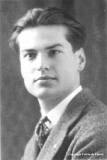
\includegraphics[width=\threefig]{\figdir/deFinetti.jpg}
%       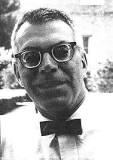
\includegraphics[width=\threefig]{\figdir/savage.jpg}
%       \caption{Bruno de Finetti (1906--1985) and L. ``Jimmie" Savage (1917--1971)}
%     \end{figure}
%   \end{itemize}
% \end{frame}

% \begin{frame}{Savage's axioms}
% \begin{itemize}
% \item Start with the triple $(\cS,\cZ,\cA\subset \cF(\cS, \cZ))$ as in \cite{Wal50}.
% \item Savage's idea is to list what we expect from a binary relation $\prec$ on $\cA\times \cA$ describing a decision maker's preferences.
% \end{itemize}
% \blank
% \blank
% \end{frame}

% \begin{frame}{Savage's axioms}
% \end{frame}

% \begin{frame}{Savage's axioms}
% \end{frame}

% \begin{frame}{A De Finetti theorem by Hewitt \& Savage}
%   \begin{block}{Theorem; see \citep[Theorem 1.49]{Sch12}}
%     Let $X_1,X_2,\dots$ be a sequence of exchangeable random variables on $\cX$, i.e.
%     $$
%     X_1,\dots,X_n \sim X_{\pi(1)},\dots, X_{\pi(n)}, \forall n, \forall \pi\in\frak S_n.
%     $$
%     Then there exists a probability distribution $\mu$ \un{on the set of probability measures $\mathcal P(\cX)$ on $\cX$} such that
%     $$
%     \mathbb P (X_1\in A_1, \dots, X_n\in A_n) = \int Q(A_1)\dots Q(A_n)\d\mu(Q).
%     $$
%     % Furthermore, for each $A$,
%     % $$
%     % Q(A) = \lim_{n\rightarrow\infty} \frac 1n\sum_{i=1}^n 1_A(X_i)\quad a.s.
%     % $$
%   \end{block}
%   \vfill
%   To a subjectivist, Savage's theorem says you should use SEU, and representation theorems like de Finetti's constrain your choice of $p$.
% \end{frame}

% % \begin{frame}{De Finetti's theorem and LDA}
% % \end{frame}

% % \begin{frame}{De Finetti's theorem and Bayesian nonparametrics}
% % \end{frame}

% \begin{frame}{Bonus: The Dirichlet process through de Finetti's theorem}

% \begin{block}{The Blackwell-McQueen urn scheme (aka the CRP)}
%   Start with an urn containing a single black ball with weight $\alpha$. Repeat: draw a ball from the urn with probability $\propto$ its weight. Then,
%   \begin{itemize}
%     \item If the ball is black, return it to the urn along with another ball of weight 1, with a \un{new color} sampled from some base measure $H$.
%     \item If the ball is colored, return it to the urn along with another ball of weight 1 of the \un{same color}.
%   \end{itemize}
%   Denote by $X_1, X_2, \dots$ the color of the ball added.
% \end{block}
% \begin{flushright}
%   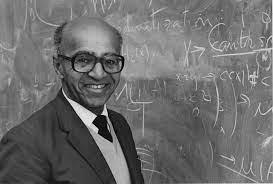
\includegraphics[width=\twofigminus]{Figures/blackwell.jpg}
% \end{flushright}
% \vfill
% % \begin{itemize}
% %   \item Exercise: show that $X_1,X_2,...$ are exchangeable.
% %   \item The corresponding prior $\mu$ on $\mathcal{P}(\cX)$ is the Dirichlet process with concentration $\alpha$ and base measure $H$.
% % \end{itemize}
% \end{frame}

% \begin{frame}{Pros and cons of the subjectivist viewpoint}
% \begin{itemize}
%   \item Axiomatic derivations are powerful, and shed light on what coherence requires. \un{In particular, coherence leads to SEU}.
%   \vfill
%   \item[\frownie] ... Yet all axiomatic systems have a bit that is difficult to swallow.
%   \vfill
%   \item Priors should be elicited by \un{expert knowledge}, and should be \emph{bona fide} probability distributions.
%   \vfill
%   \item Representation theorems can help design the joint distribution over states \citep{OrRo14}.
%   \vfill
%   \item Bayesian nonparametrics has revived the subjectivist viewpoint.
% \end{itemize}

% \end{frame}
